\chapter{Planificación de caja}\label{chp-04}

Para que todos los dispositivos que componen el sistema estén bien aislados del exterior
y no haya problemas con las conexiones se planifica una caja estanca. Ésta deberá ser 
accesible para el reemplazo de dispositivos defectuosos y ser replicable. 

\section{Diseño de caja}

Como referencia se toma de una caja de dimensiones 220 x 145 x 80 mm. Para reducir los 
costes, se decide imprimirla en 3D, ya que permite mayor adaptabilidad para colocar 
los lugares donde fijar los diferentes dispositivos. La caja estará dividida en una base y una 
tapa que se unen mediante tornillos y permiten una unión estable.

\subsection{Base}

La base debe tener las siguientes características:
\begin{itemize}
    \item Permitir fijar y extraer con facilidad todos los dispositivos. 
    \item Orificio para entrada de cables de conexión.
    \item Hueco para conector hembra Ethernet.
    \item Hueco para conector de pines digitales.
\end{itemize} 

Con todo ello se ha diseñado la base que se puede ver en la figura \ref{fig:cajabase}. Se muestra
una imagen de la planta y otra general. Se puede observar que cuenta con distintos orificios en los
que se debe introducir tuercas M3 durante la impresión en 3D para los distintos anclajes de dispositivos
que se comenta a continuación y para la unión con la tapa para que quede estanca la caja.

Además, para el anclaje de los dispositivos sobre la base, se ha diseñado un soporte que va atornillado
a la misma. Para ello, se ha modelado de forma simplificada todos los dispositivos y se ha buscado la 
forma óptima de disponerlos. También se ha tenido en cuenta los cables que van conectados tanto a la 
fuente como al Arduino, modelándolos en el espacio que ocupan hasta que el ángulo de giro es aceptable
para que el cable se pueda colocar de forma holgada y sin tensiones dentro de la caja.
Posteriormente se ha creado el soporte en base a dicha disposición y contando con los orificios de cada
dispositivo. En la figura \ref{fig:ensamblajebase} se puede ver el resultado final de este ensamblaje.

\newpage

\begin{figure}[htpb]% 
    \centering 
    \subfloat[][]{% 
        \label{fig:cajabasevista}% 
        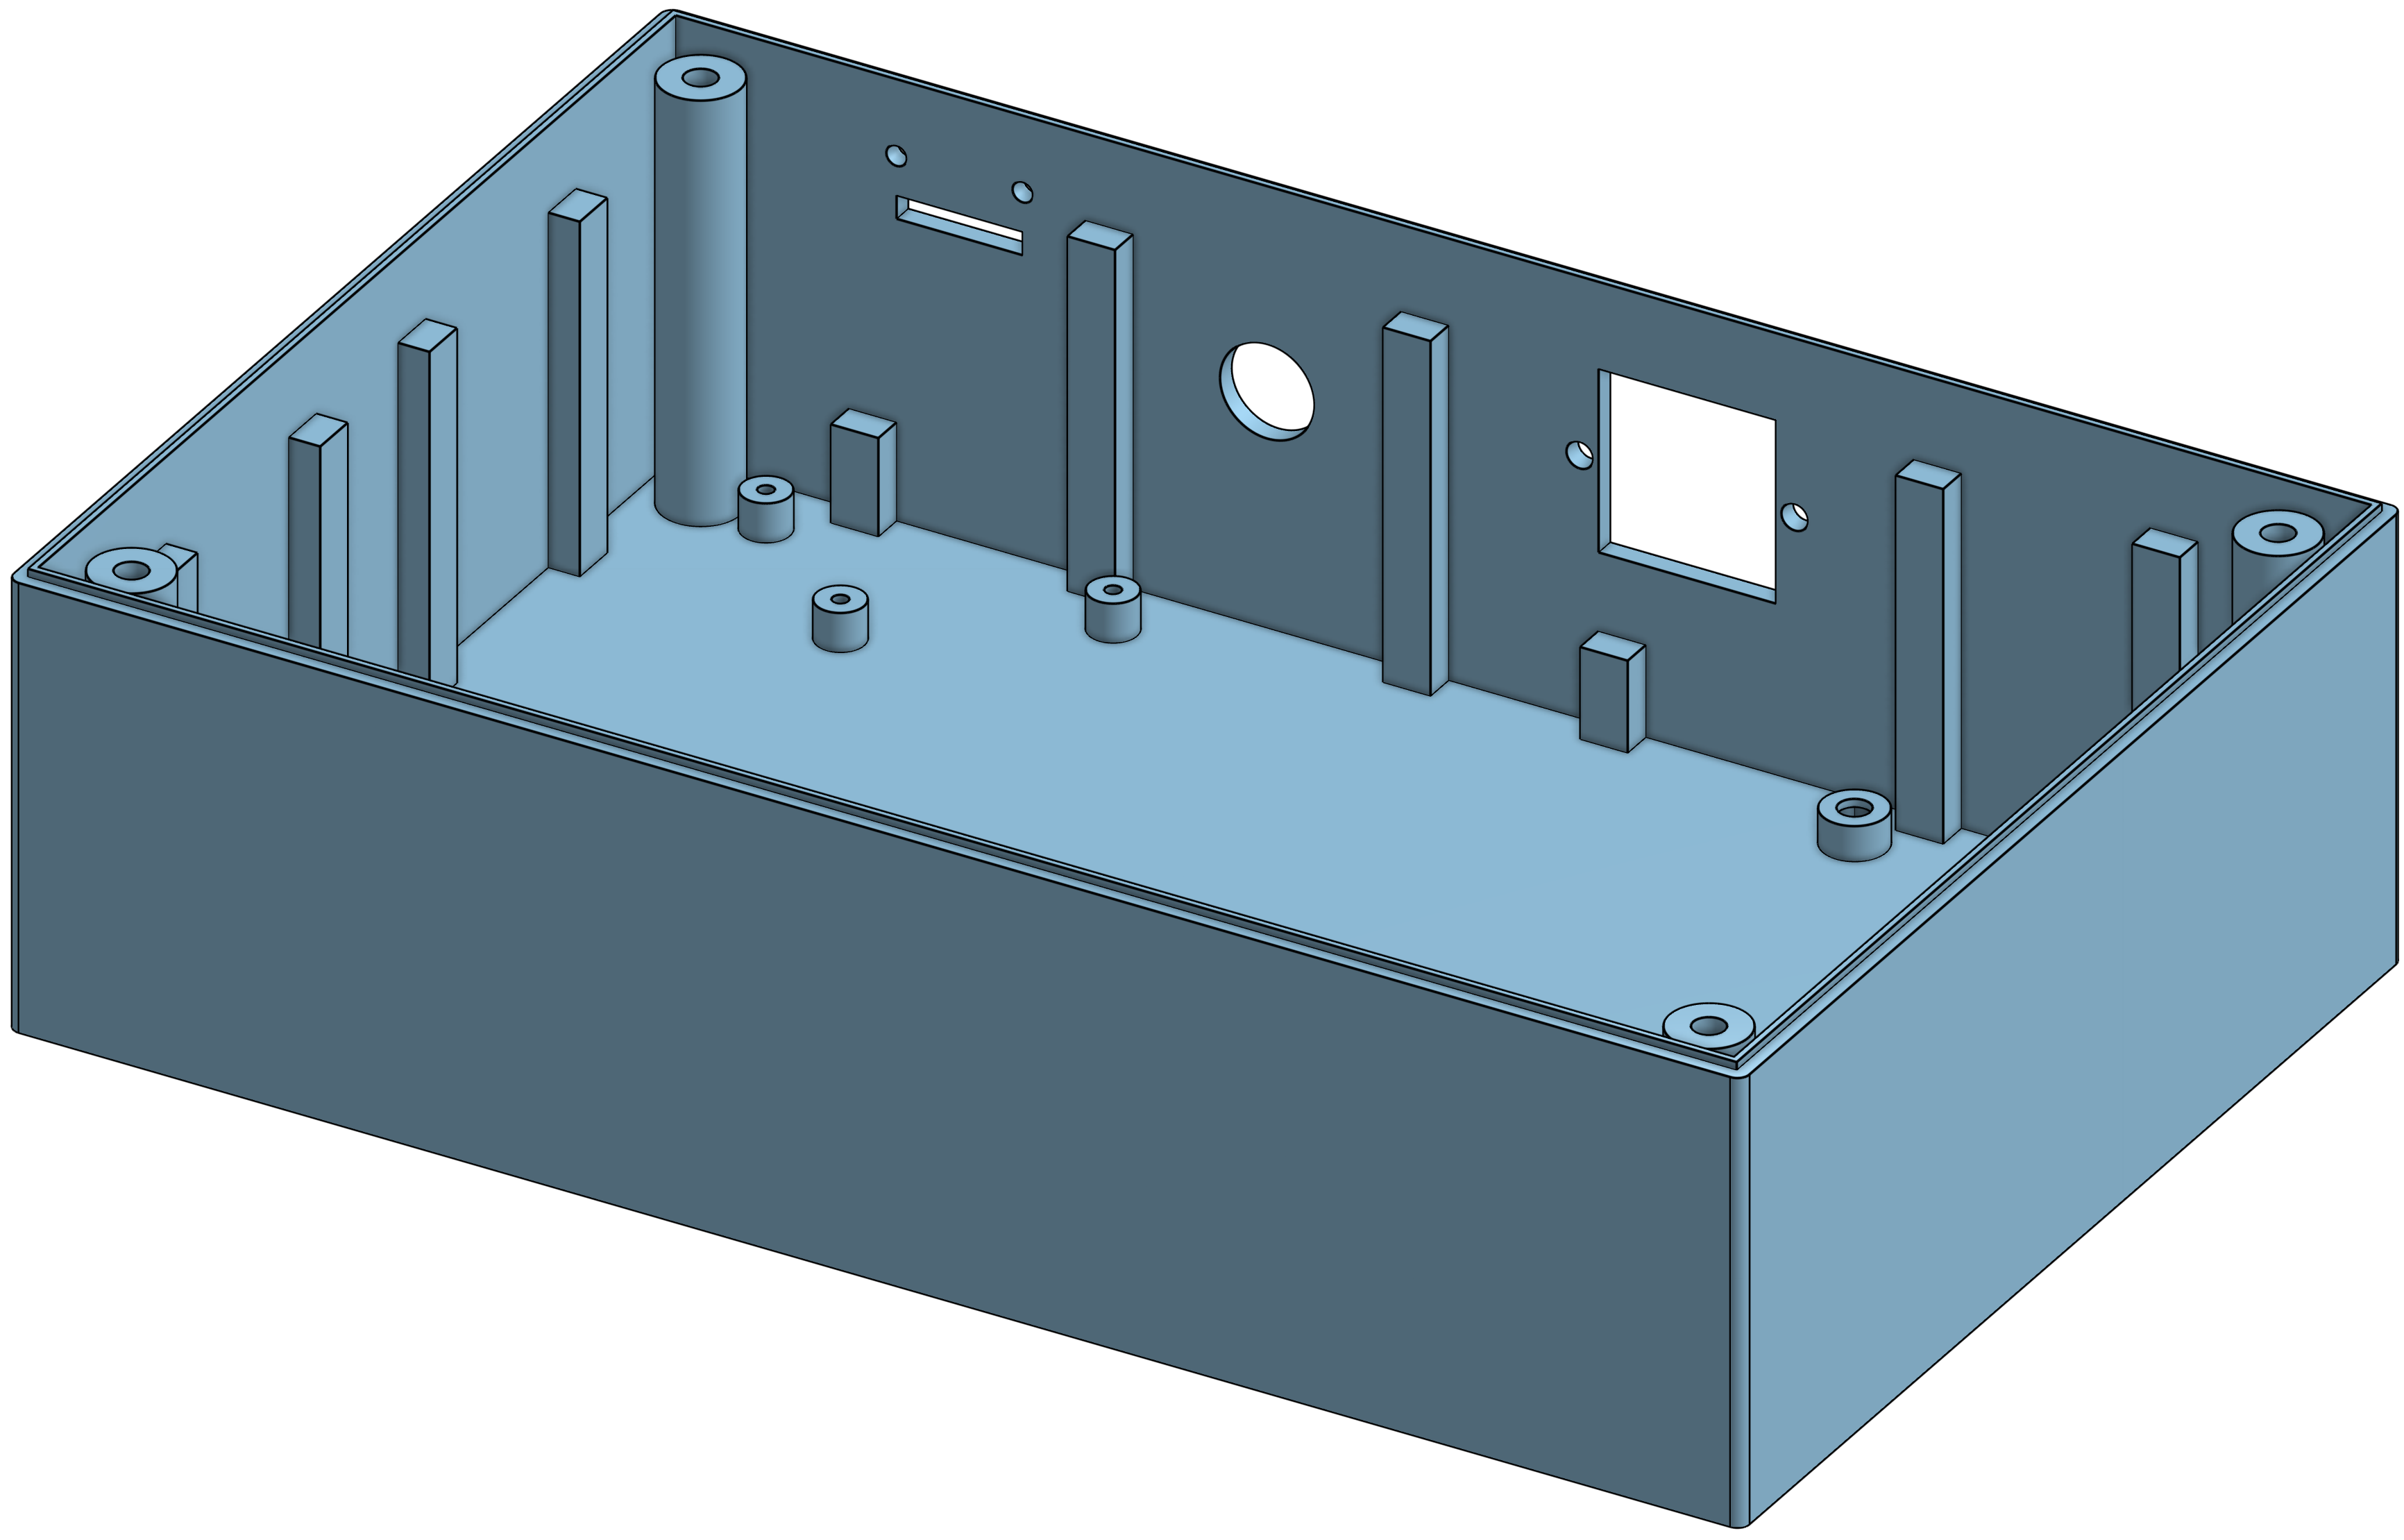
\includegraphics[width=\textwidth/2]{04-caja/cajabase.png}
    }% 
    \hspace{10pt}% 
    \subfloat[][]{% 
        \label{fig:cajabaseplanta}% 
        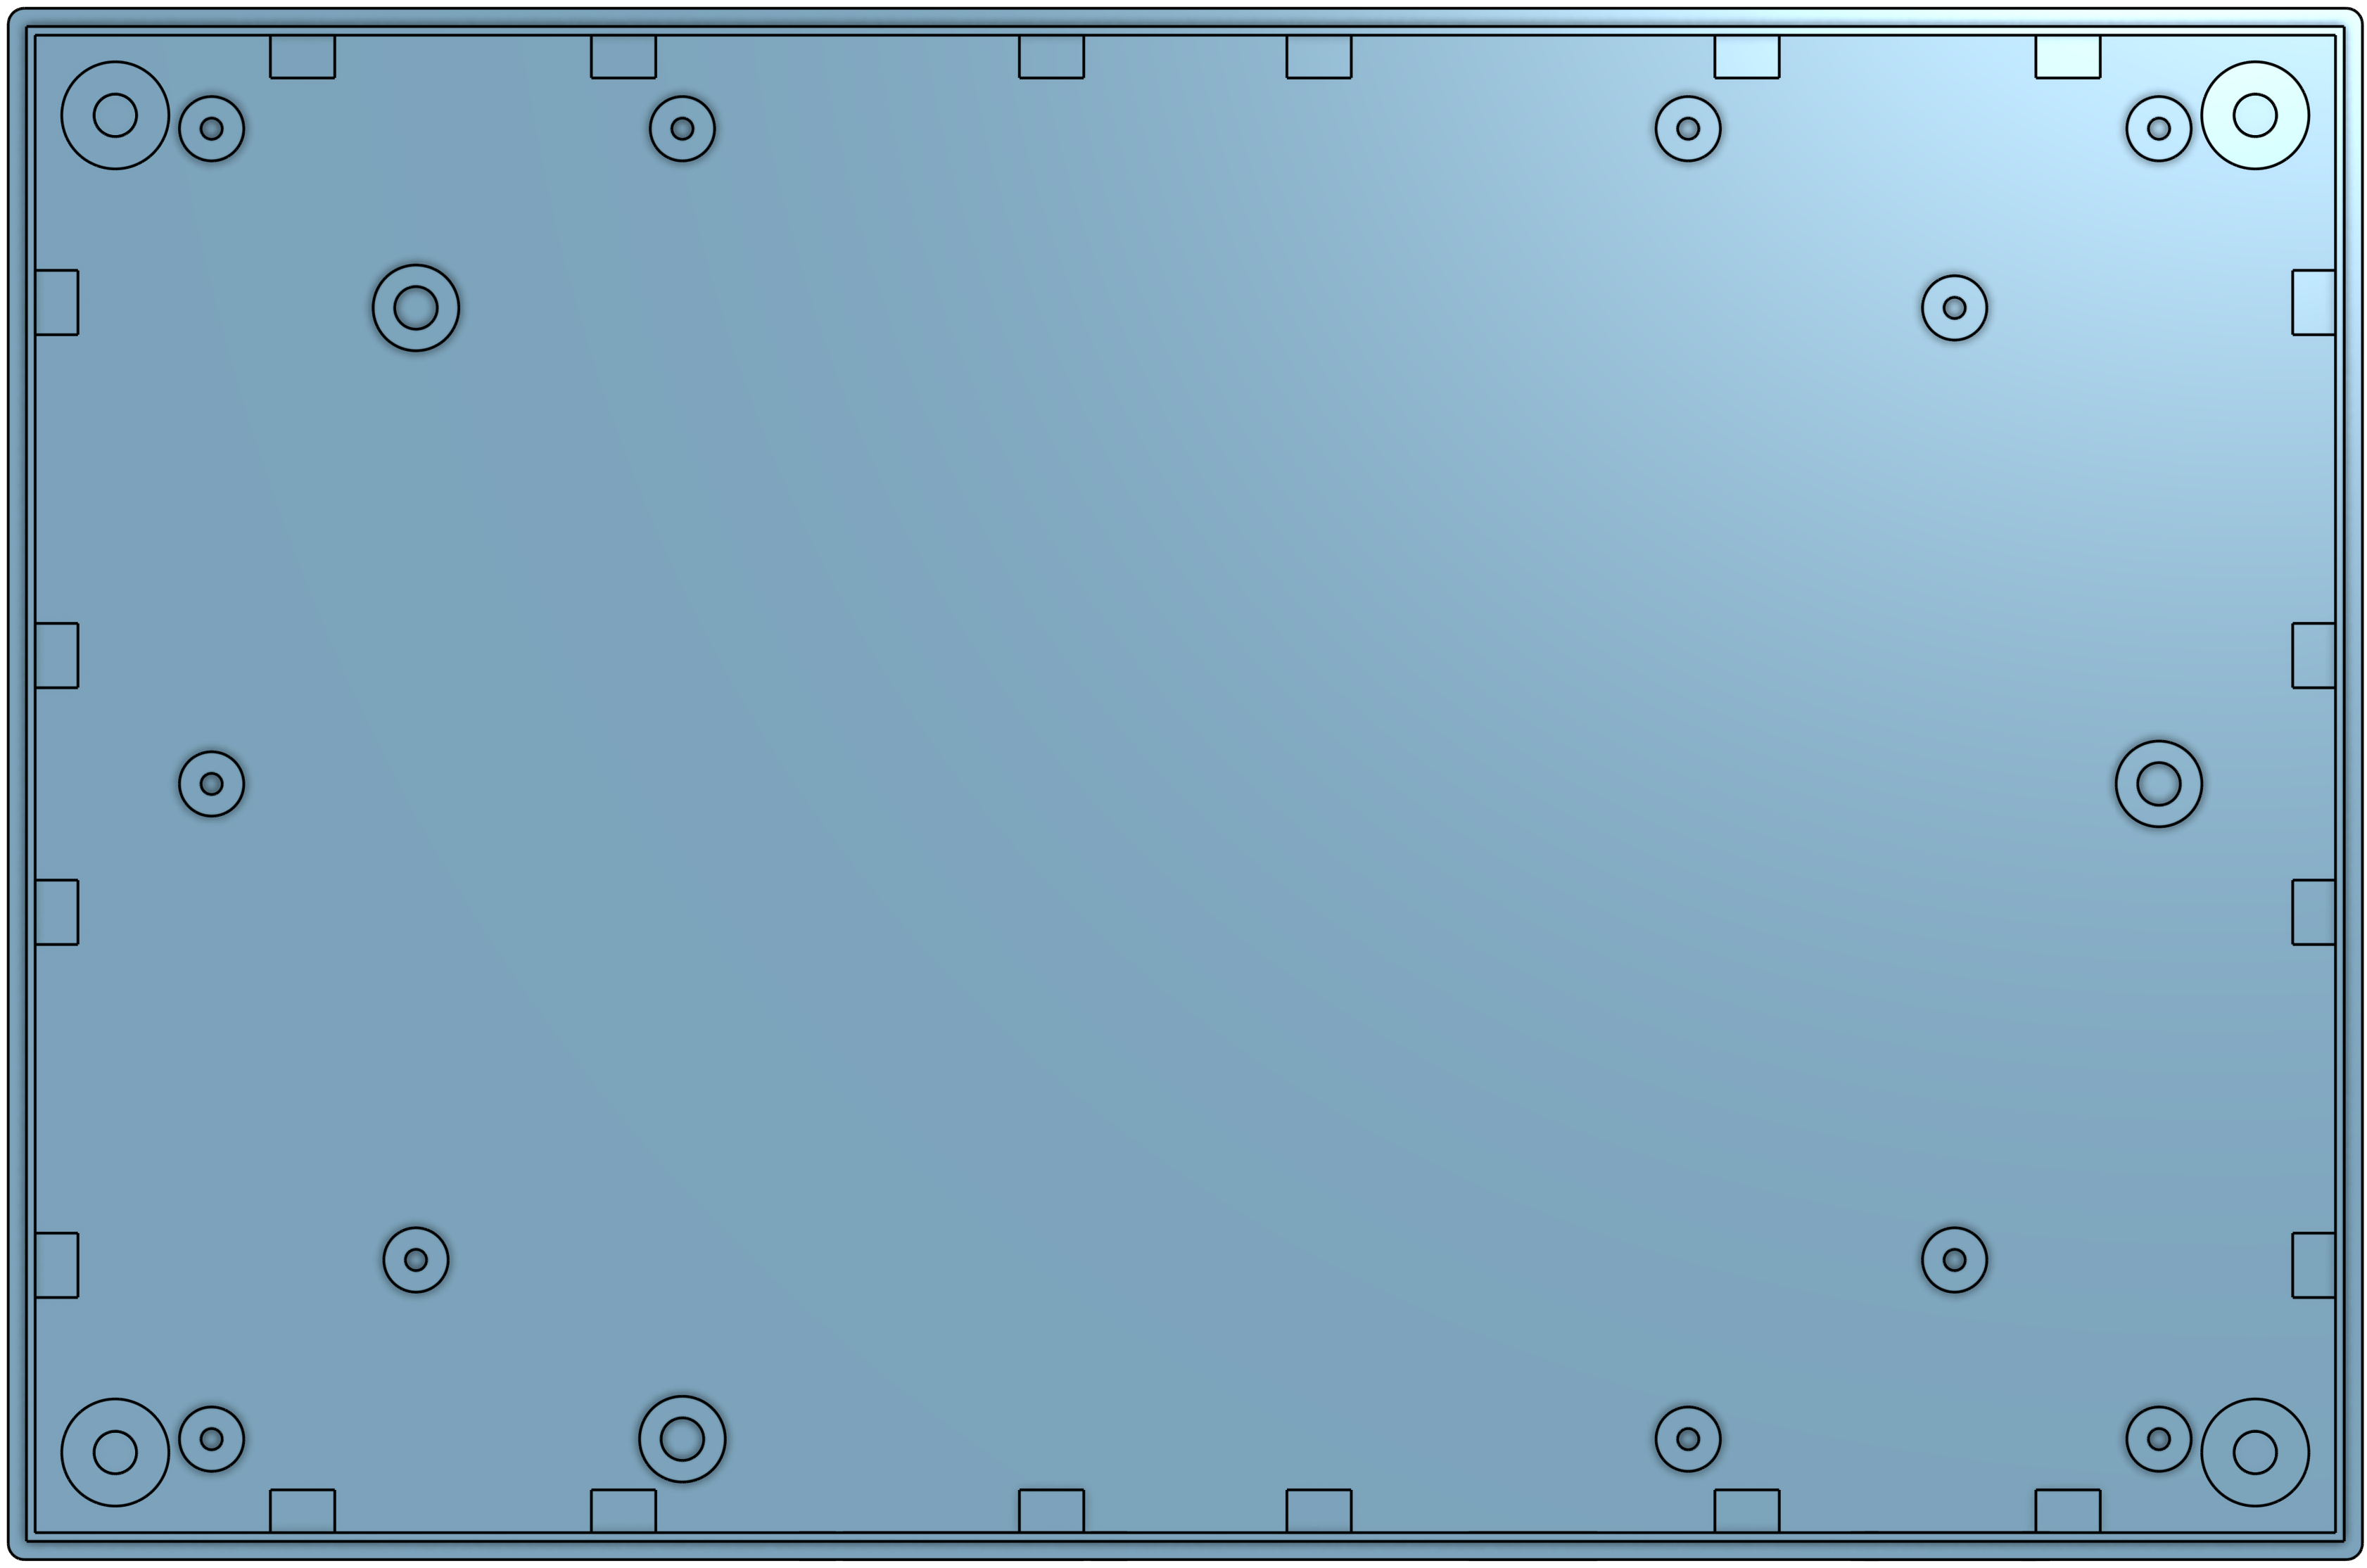
\includegraphics[width=\textwidth/2]{04-caja/cajabaseplanta.png}
    }
    \caption{a) Vista general de la base de la caja. b) Vista de planta de la base de la caja}
    \label{fig:cajabase} 
\end{figure} 


\begin{figure}[hbtp]
    \centering
    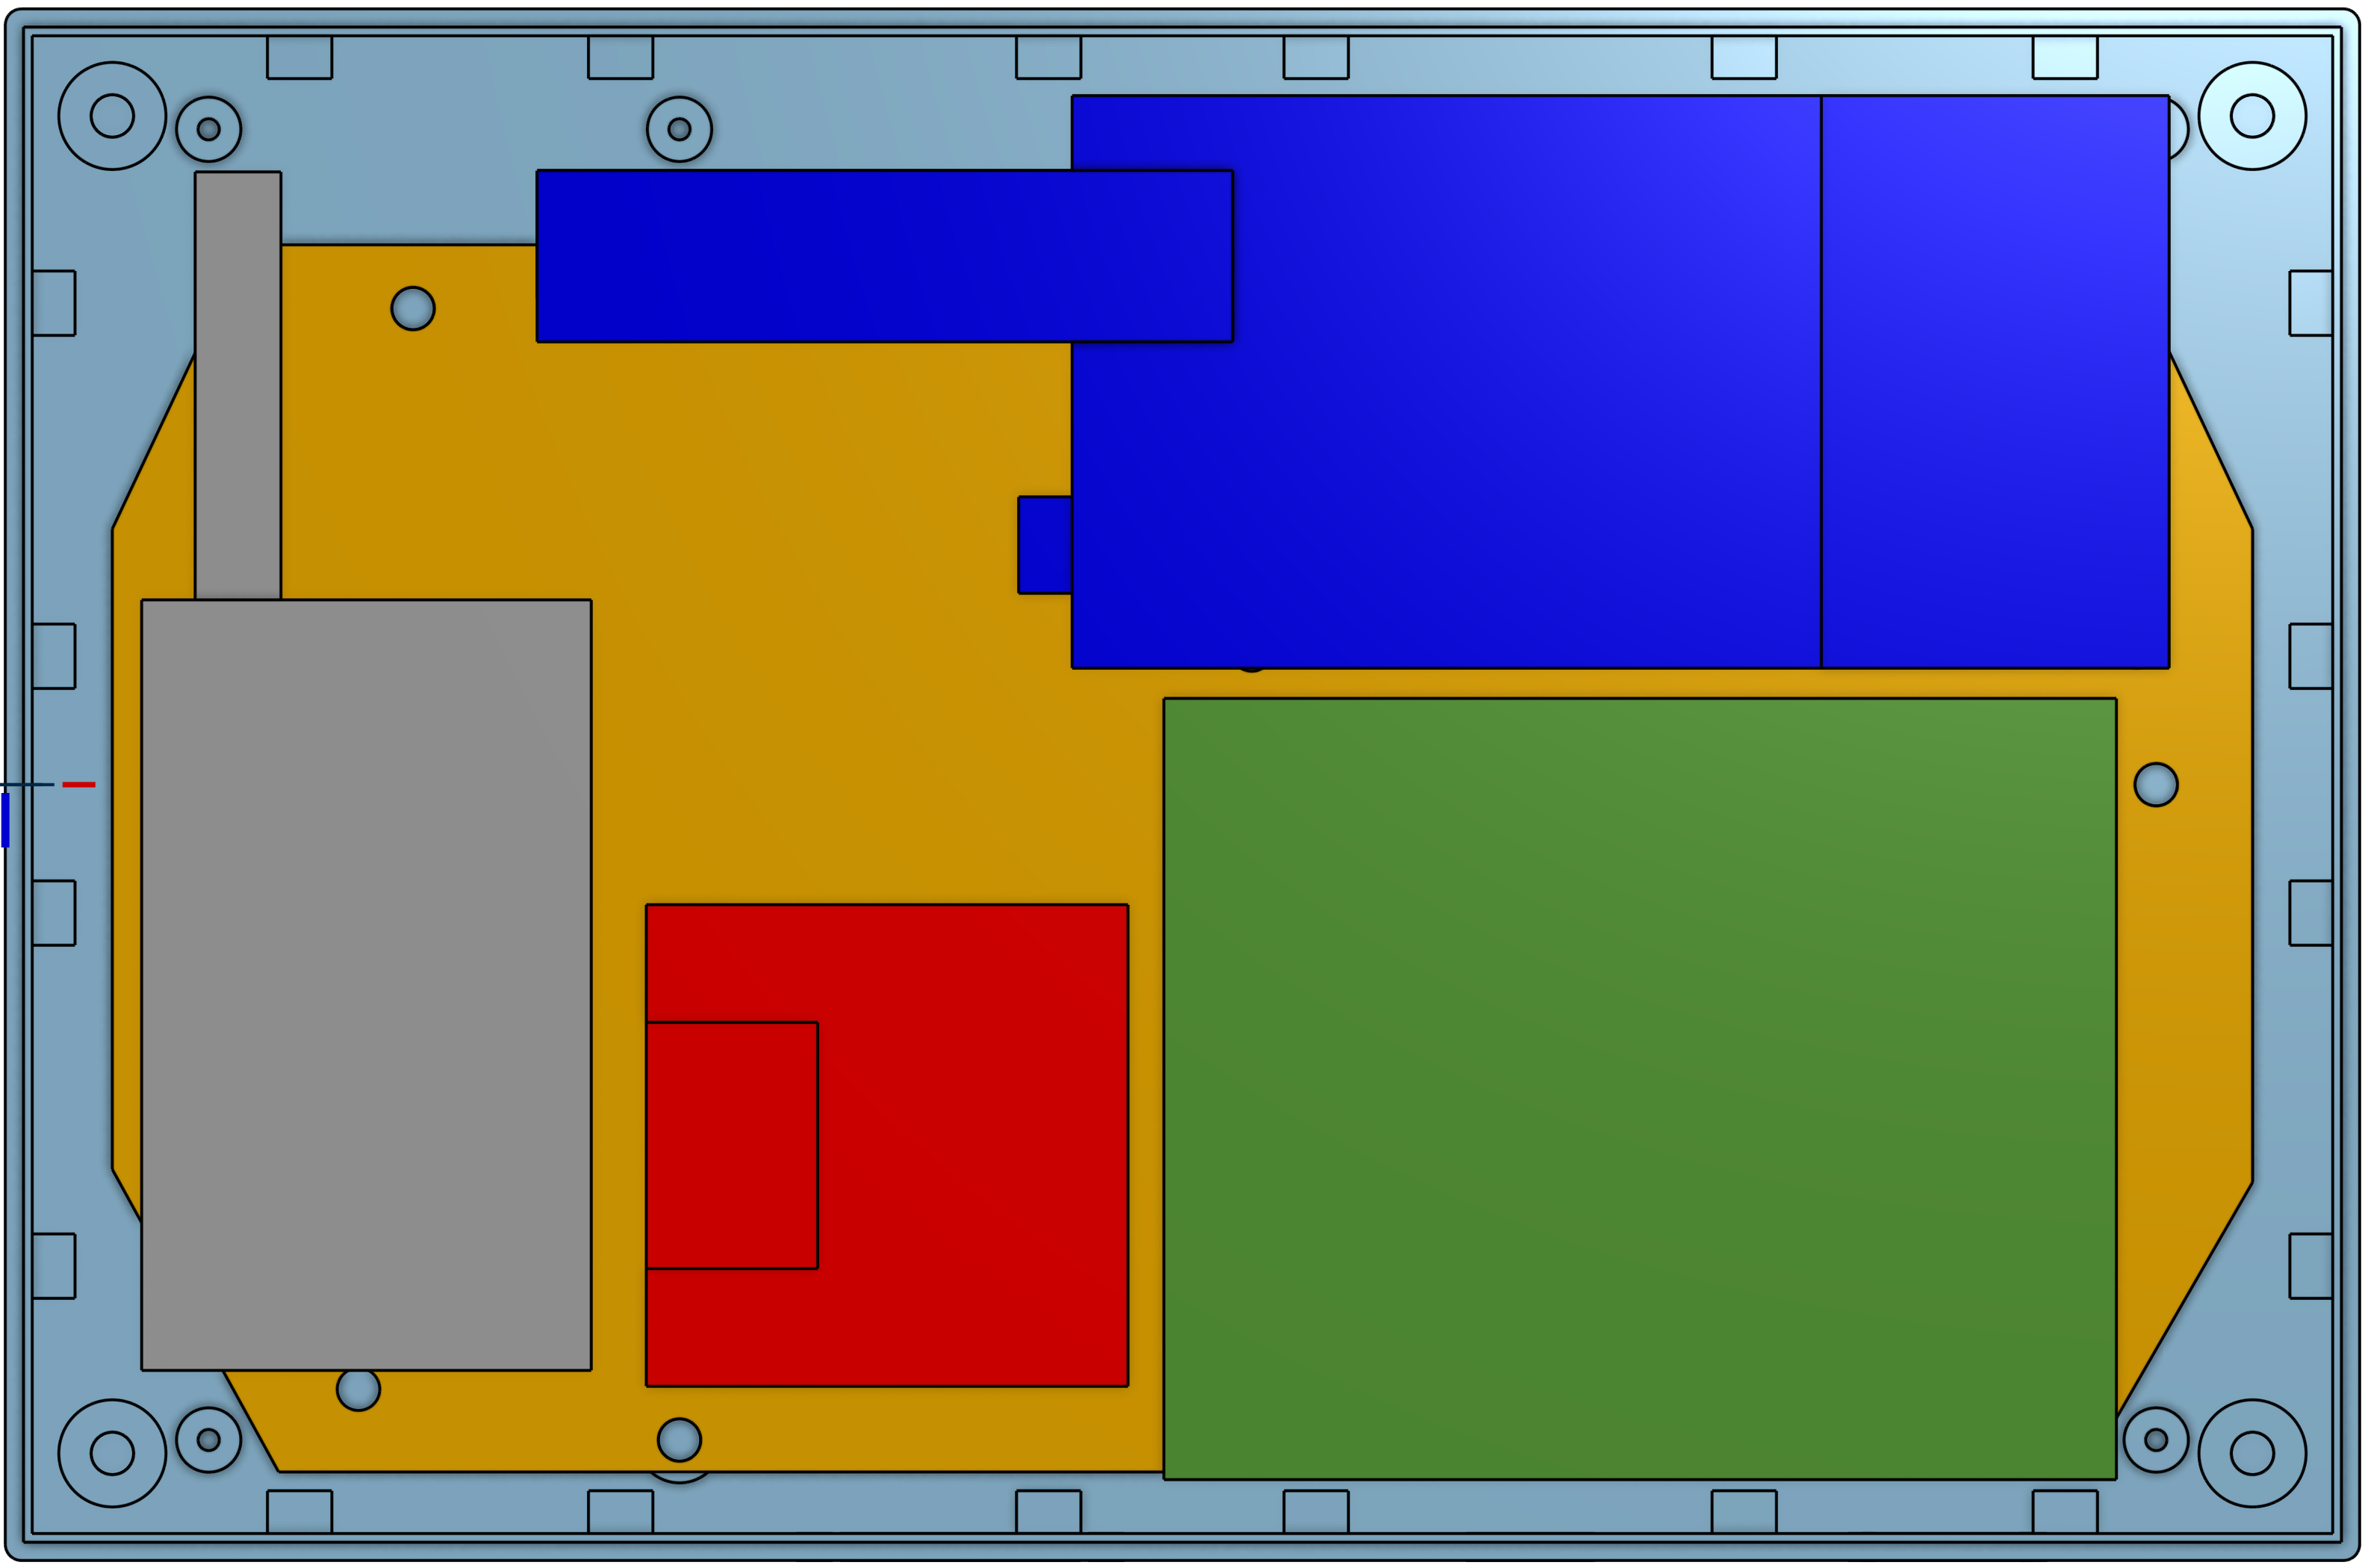
\includegraphics[width=\textwidth/2]{04-caja/ensamblajebase.png}
    \caption{Ensamblaje de la base con el soporte. Descripción por colores: a) Gris: Fuente. 
    b) Rojo: L298N. c) Azul: Arduino. d) Verde: placa de conexiones. e) Amarillo: Soporte tapa}
    \label{fig:ensamblajebase}
    \end{figure}


\subsection{Tapa}
Bebé a bordo.

\begin{figure}[htpb]% 
    \centering 
    \subfloat[][]{% 
        \label{fig:cajatapavista}% 
        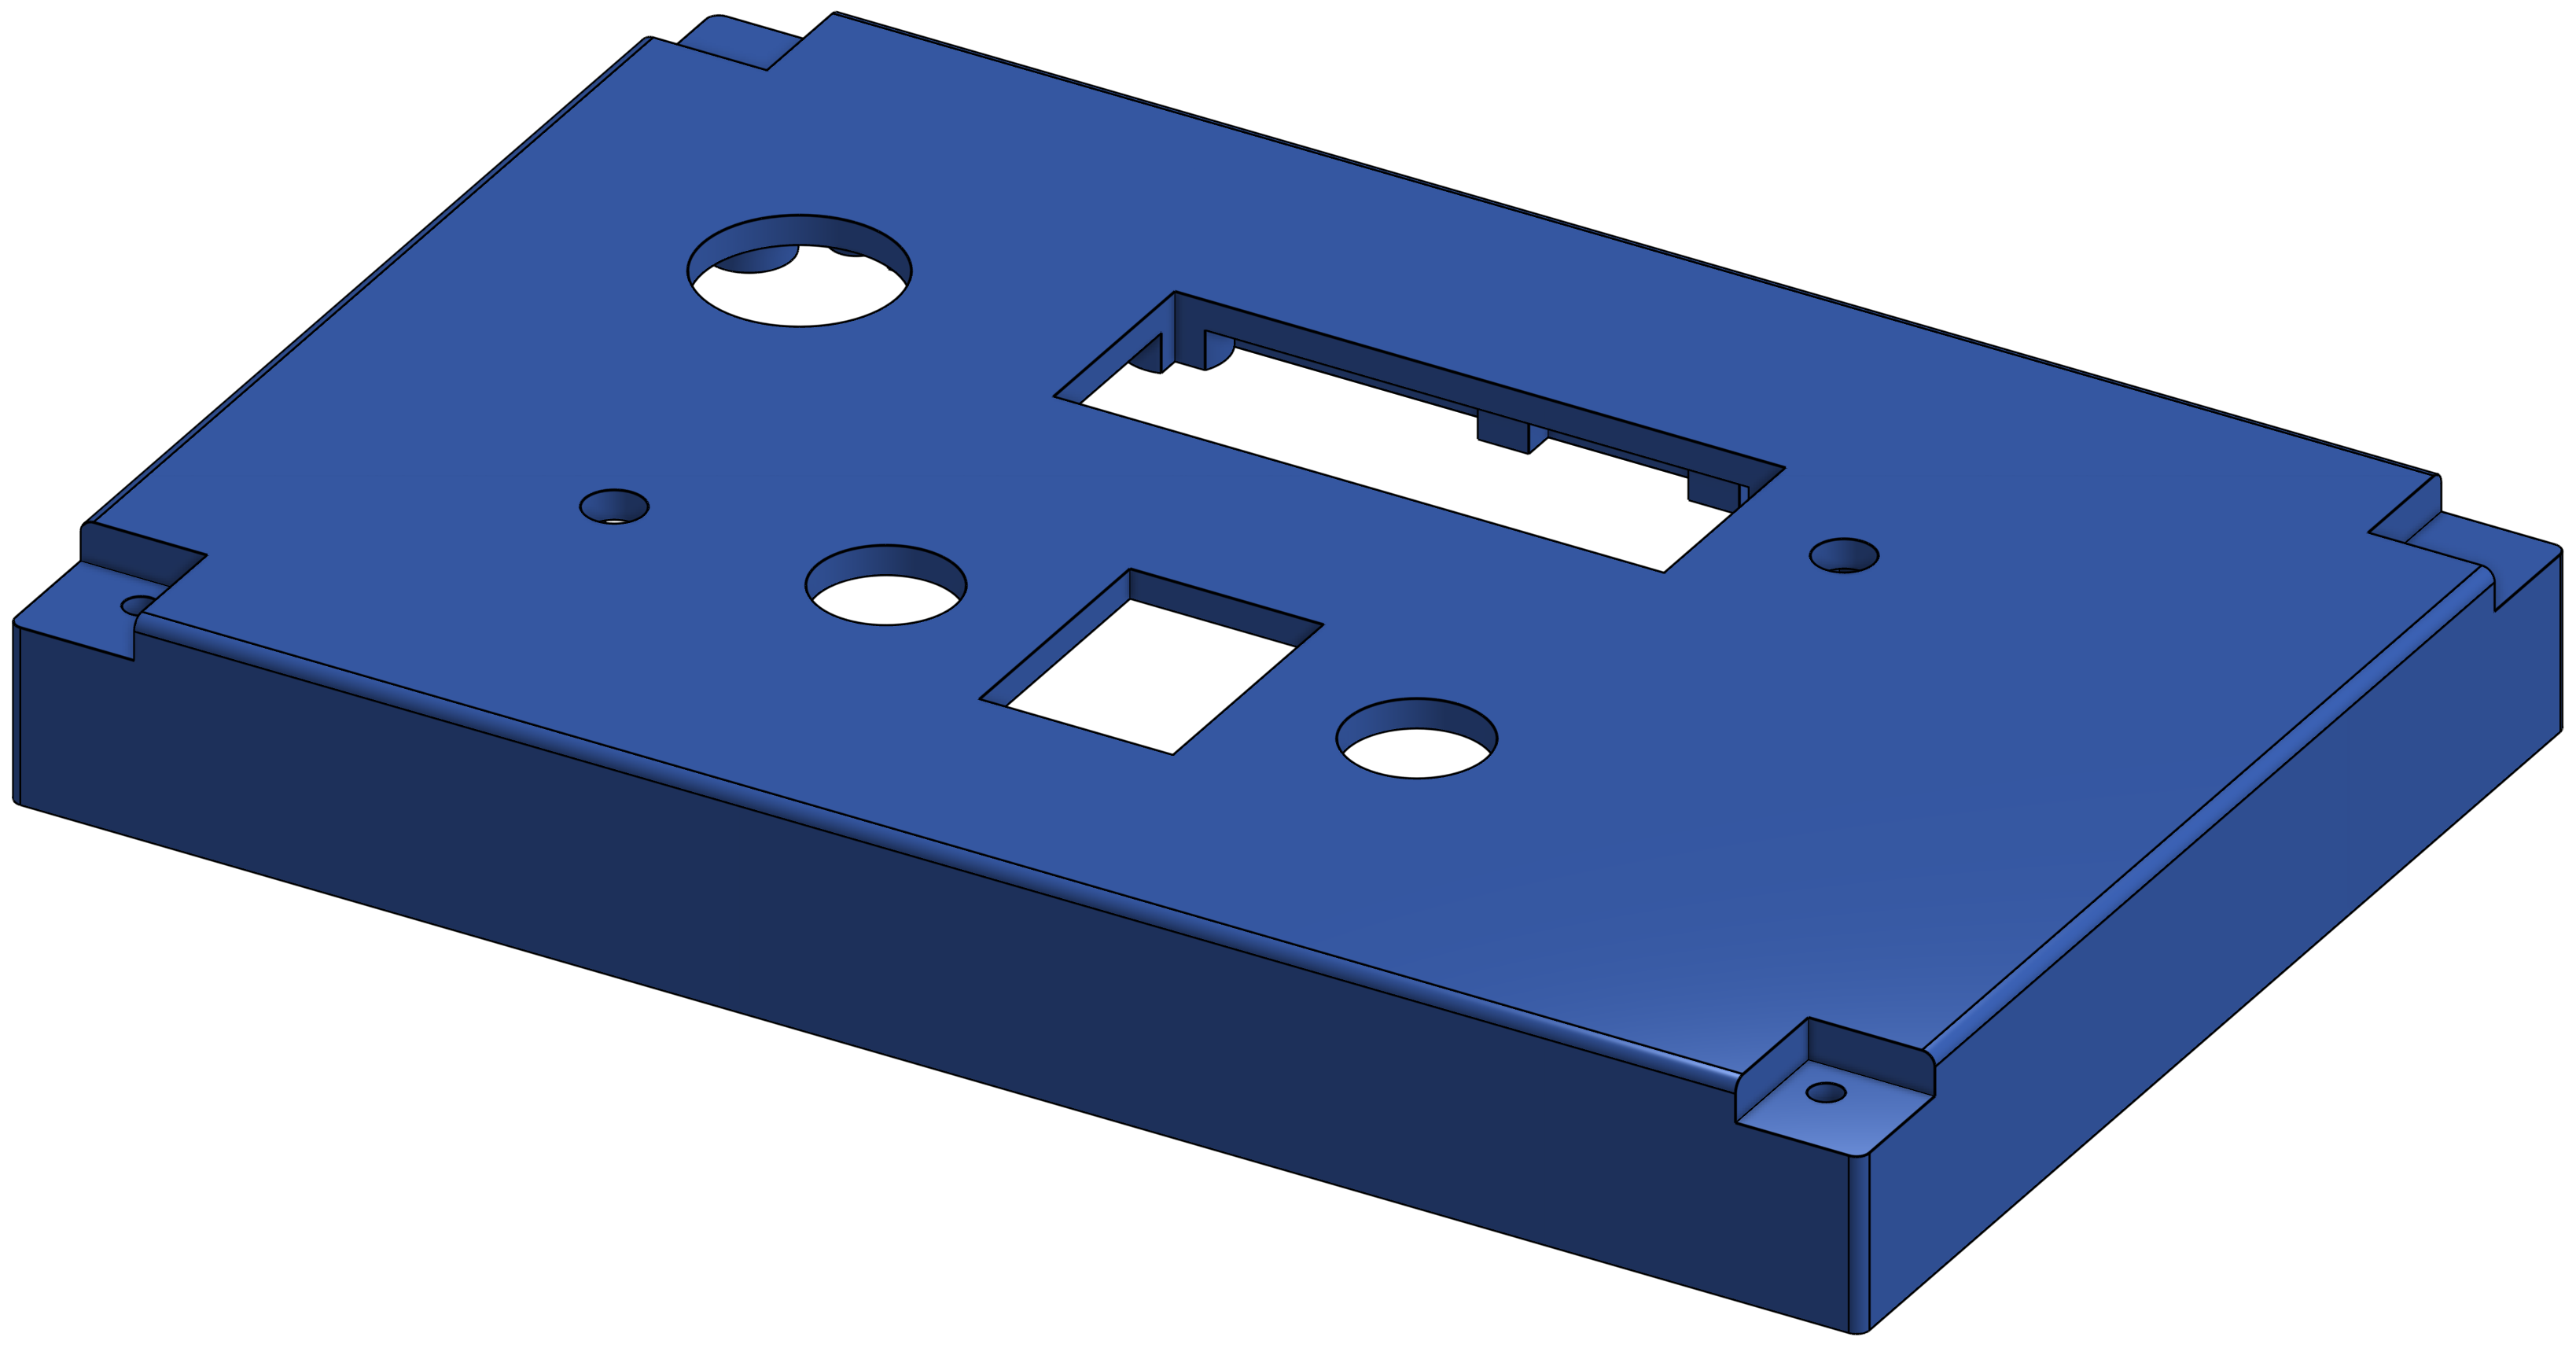
\includegraphics[width=0.75\textwidth]{04-caja/cajatapa.png}
    }% 
    \hspace{10pt}% 
    \subfloat[][]{% 
        \label{fig:cajatapaplanta}% 
        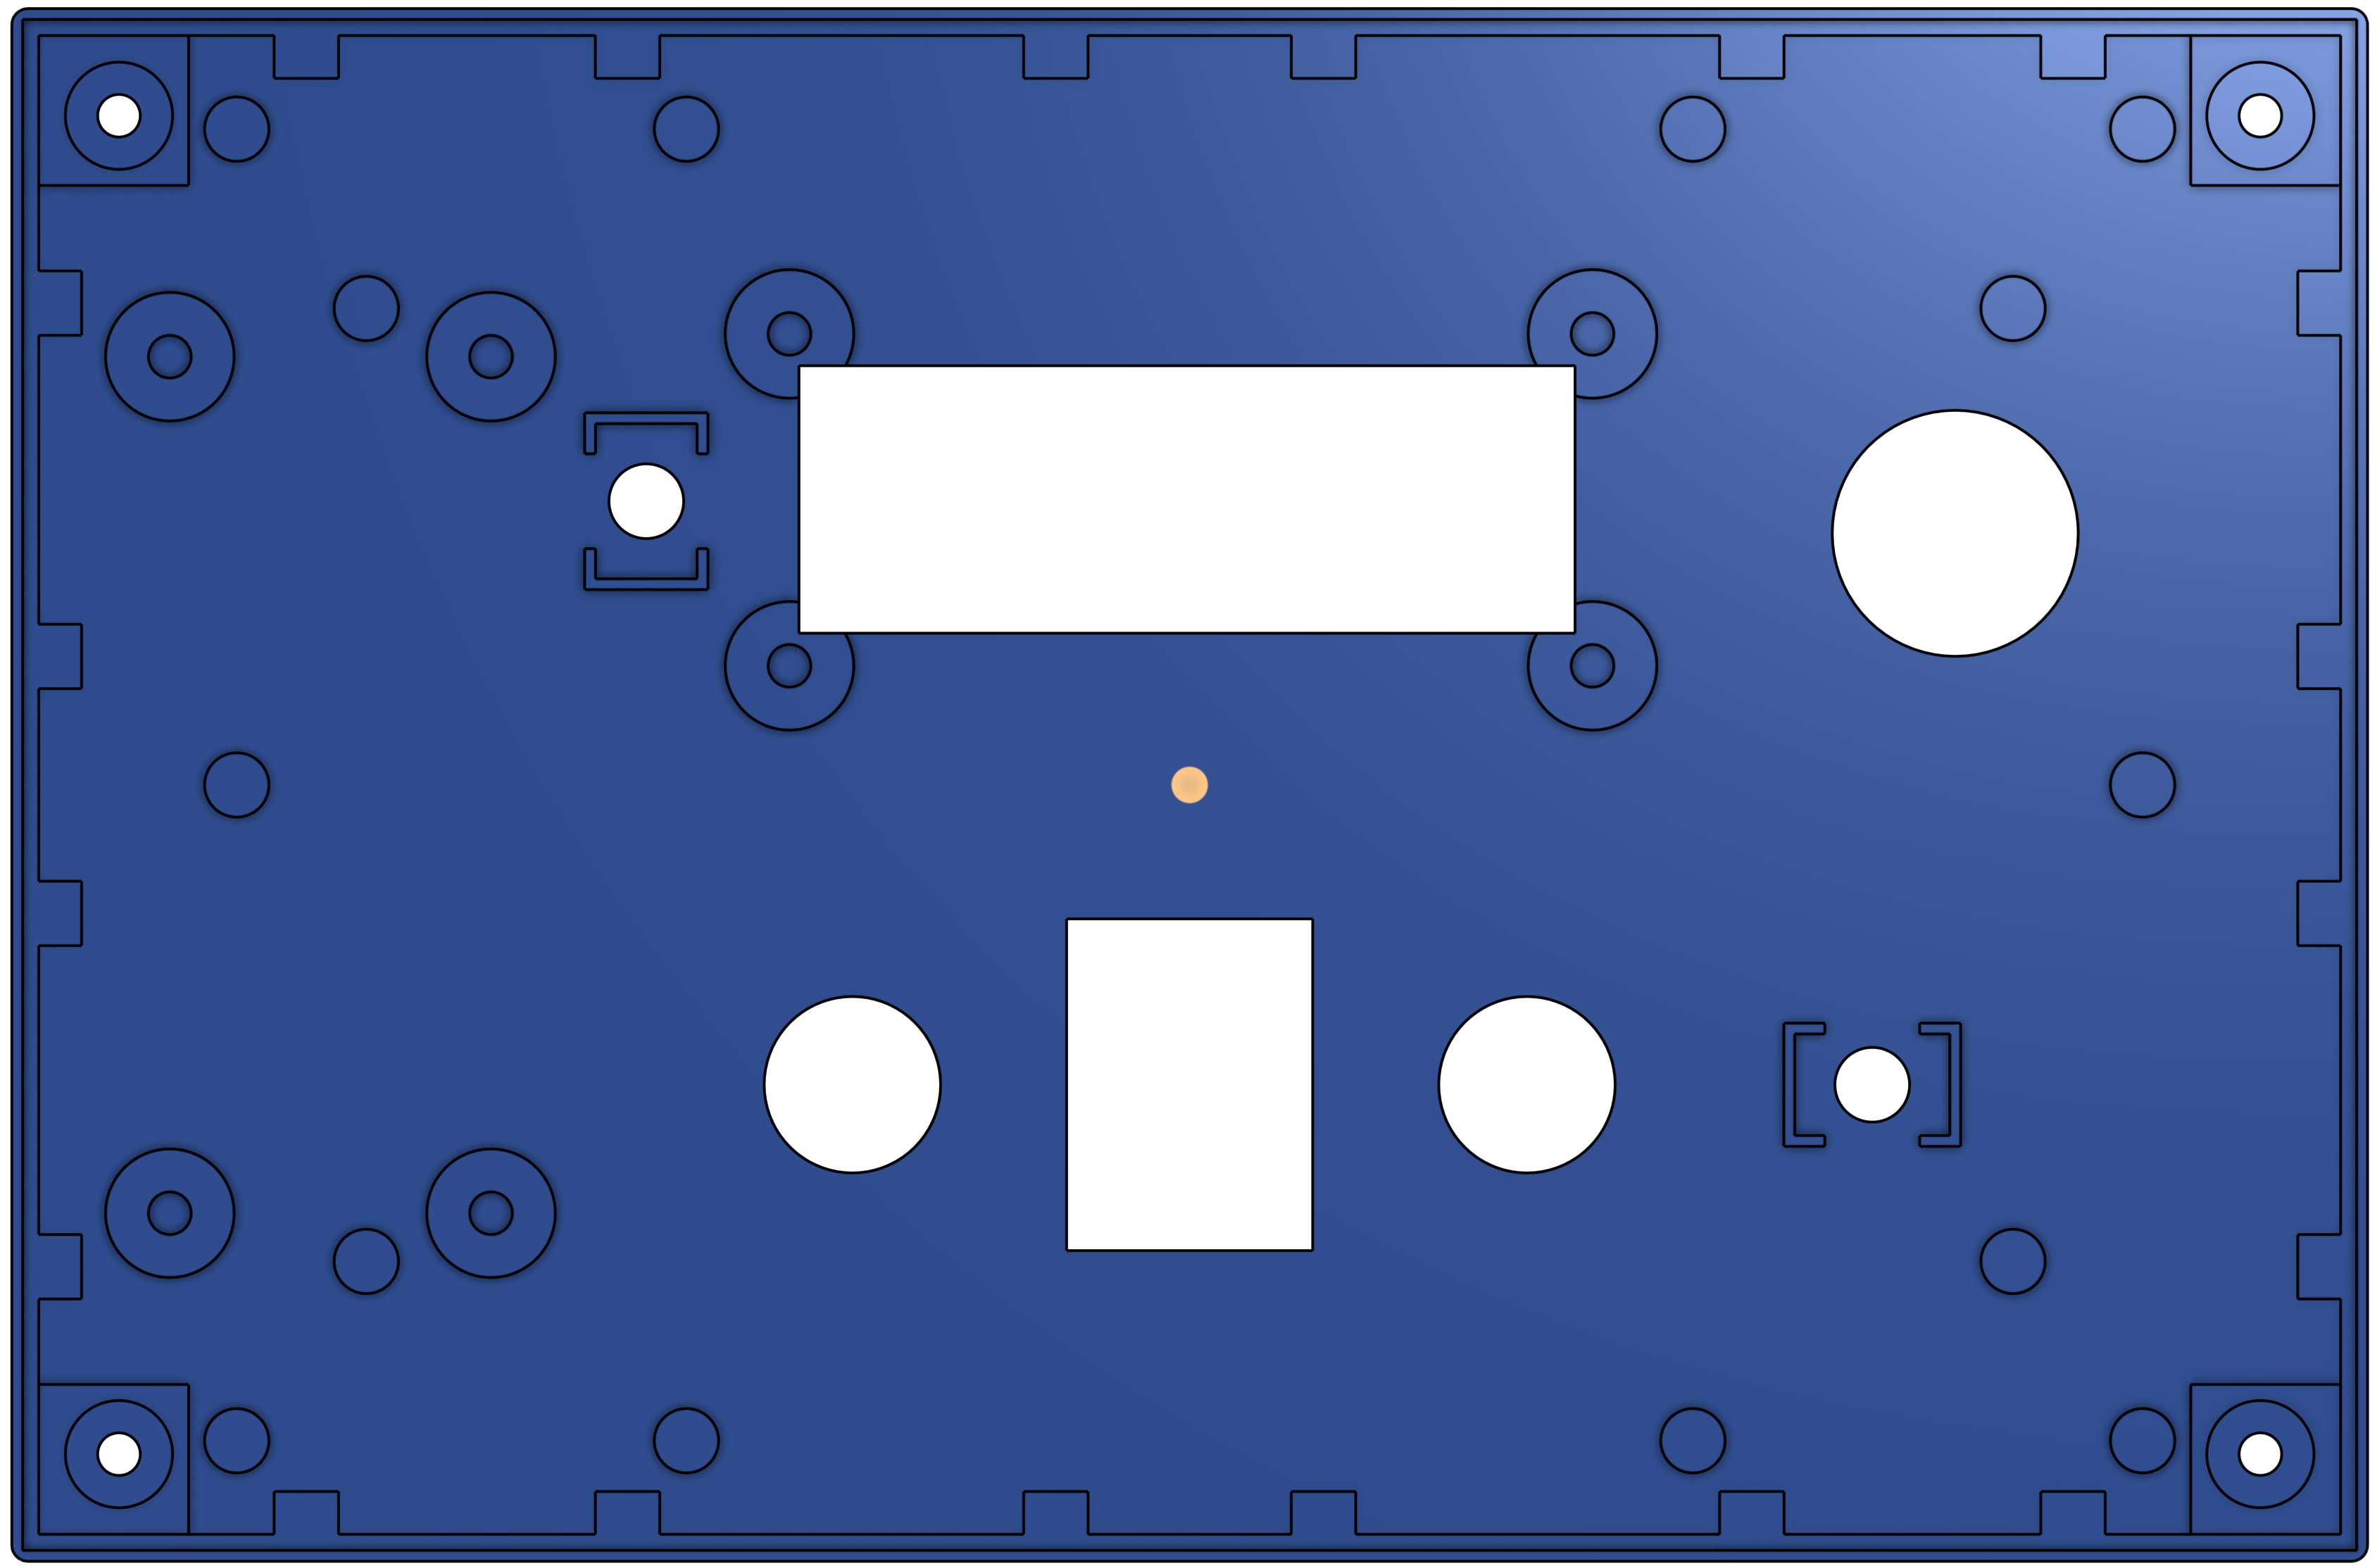
\includegraphics[width=0.75\textwidth]{04-caja/cajatapafondo.png}
    }
    \caption{a) Vista general de la tapa de la caja. b) Vista inferior de la tapa de la caja}
    \label{fig:cajatapa} 
\end{figure} 
